\section{Challenges and Design Highlights} \label{sec:scalims-motivation}

%\noindent \textbf{Motivation.}
%The key motivation of this study is the fact that there are no NFV scaling systems designed to operate under a multi-datacenter environment, given the following new challenges compared with scaling service chains within a single datacenter.
\textit{ScalIMS} aims to address the following challenges, that arise when scaling service chains over multiple datacenters.

{\em First, deciding service chain paths}, as determined by the datacenters where instances of VNFs in a service chain should be deployed. The service chain path critically decides service quality of user traffic along the chain.
For instance, a traffic flow sent by a user of the IMS system to another user may have two optional paths. The first path traverses a sequence of datacenters $(a, c)$ while the second path traverses datacenters $(a, b, c)$. %Due to the triangle inequality which is a common phenomena in computer network \cite{wang2007towards}, it is possible that the accumulated delay on the second path is way smaller than that on the first path.
The end-to-end delays on the two paths may vary over time. A multi-datacenter NFV scaling system should constantly update the service chain paths, so that a good service quality can be guaranteed for user traffic at all time.
%In Fig.~\ref{fig:system-overview}(a), the flow %traffic of IMS system user can go through either one of the two service chain paths (containing two VNFs each).The lower path leads to a 50ms end-to-end delay while the upper one 100ms.


{\em Second, deciding scaling in/out of network functions}, i.e., adding/removing instances of each VNF upon traffic rise/drop. This decision is coupled with service chain path selection in the multi-datacenter setting. If a service chain path is  overloaded, instead of launching new VNF instances on the same datacenters, the system may search for available VNF instances on other datacenters, and set up new service chain paths using those instances. %This need stands out from the existing studies dealing with a single datacenter, where scaling is achieved through launching new VNF instances only.

{\em Third, distributed flow routing}. %Using SDN to control flow routing in a data center is a common approach adopted by the existing scaling systems. However,
When a service chain path traverses multiple datacenters, it is difficult for a single controller to control the end-to-end route. % due to the lack of support for SDN-like mechanisms over the WAN.
 When multiple SDN controllers are employed in different datacenters, they should work in coordination on constant updates of service chain paths, and correctly route user traffic towards destinations.

%\noindent\textbf{Highlights of {\em ScalIMS}.}
We make the following design decisions in \textit{ScalIMS}. A functional overview of \textit{ScalIMS} is given in Fig.~\ref{fig:system-overview}.

\begin{figure}[!h]
      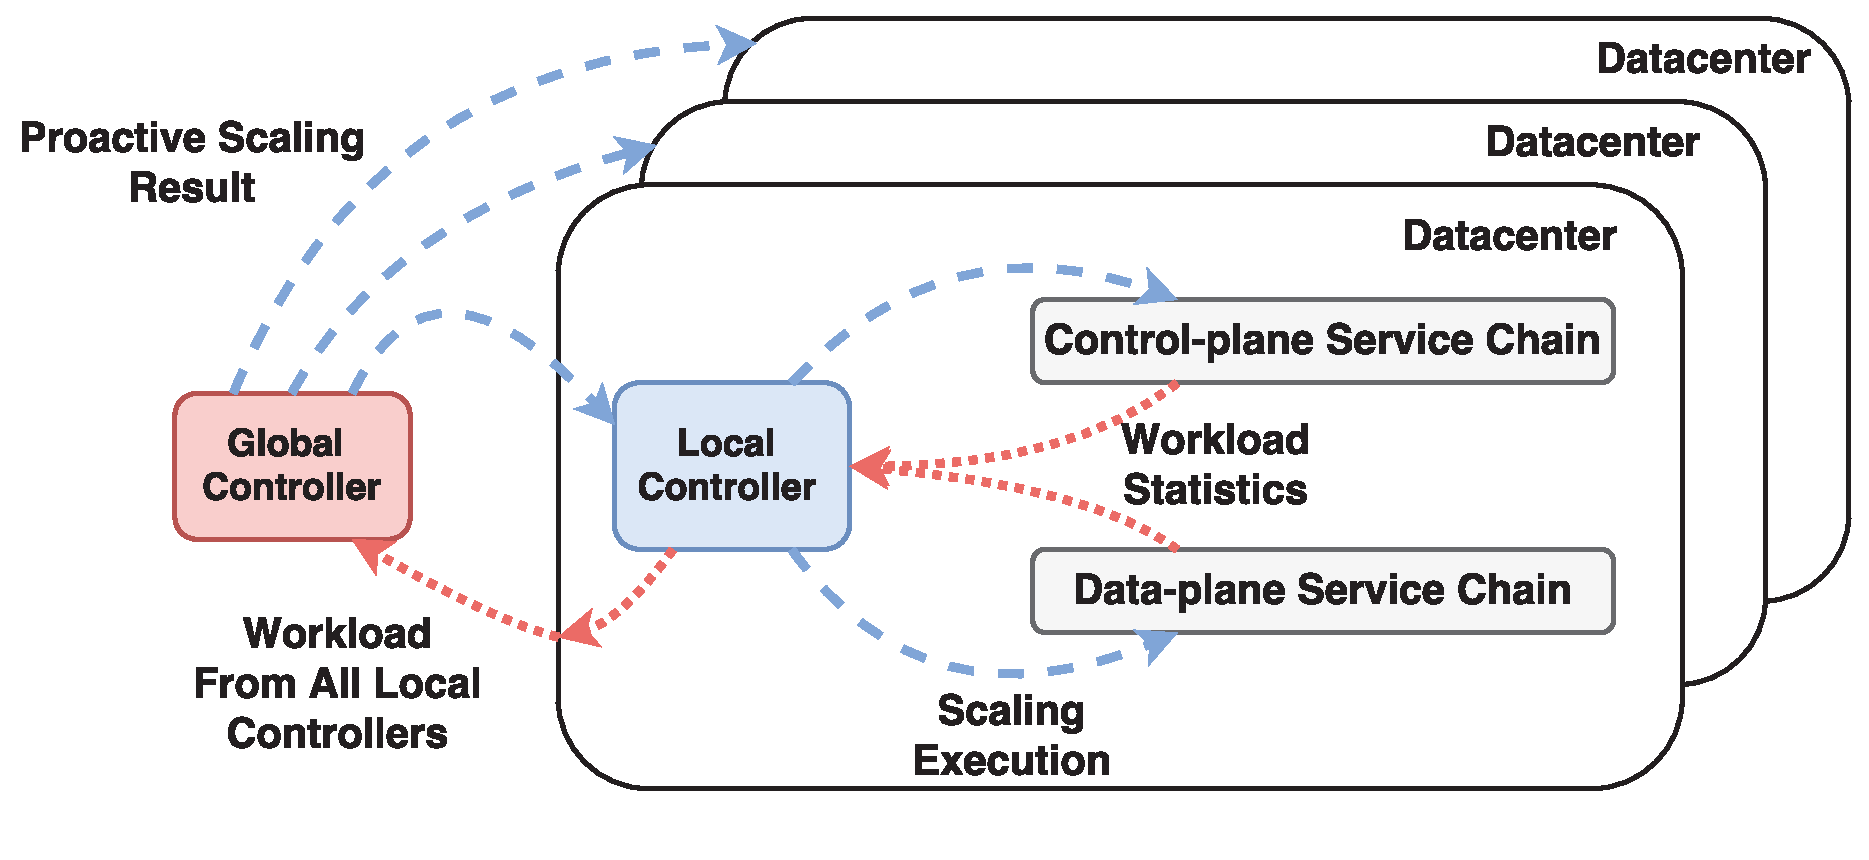
\includegraphics[width=\columnwidth]{chap-scalims/figure/scalims-overall-arch.eps}
    \caption{Functional overview of \textit{ScalIMS}}%: an overview
    \label{fig:system-overview}
\end{figure}

$\triangleright$ We adopt a hybrid scaling strategy, that combines proactive scaling and reactive scaling for both CP and DP service chains. We divide the system time into \textit{scaling intervals}. At the end of each scaling interval, proactive scaling is invoked, which takes as input the predicted workload along each service chain, inter-datacenter latencies and the current VNF deployment (the numbers of instances of each VNF on each datacenter), and generates decisions on VNF scaling and service chain path deployment with bounded end-to-end delay simultaneously for the next scaling interval. Reactive scaling produces scaling decisions of each VNF based on runtime statistics of each instance within each data center. It compensates for the inaccuracy of workload prediction with proactive scaling, improving system performance under unpredicted traffic rate changes.


$\triangleright$ \textit{ScalIMS} enables a synergy of global and local controllers, to best execute the hybrid scaling strategy. The global controller runs on a standalone server. The local controllers are SDN controllers in each data center. For proactive scaling, the global controller coordinates with all local controllers: it collects statistics from each local controller, including CPU/memory usage and network traffic volume, runs the proactive scaling algorithm, generates scaling/deployment decisions, and broadcasts the decisions to local controllers. Each local controller executes the received decisions by launching new VNF instances and adjusting service chain paths. For reactive scaling, a local controller collects runtime statistics from each VNF instance running in its datacenter, and produces local, reactive scaling decision. For flow routing, a local controller uses flow tags and service chain paths received from the global controller to determine the VNF instances that a flow should traverse within its datacenter and be dispatched to in other datacenters.


%cut for space
%$\triangleright$ We bound the end-to-end delays on service chain paths to guarantee good end-to-end performance of flows. We make some design decisions specifically tailored for an IMS system, {\em e.g.}, saving address information carried in the SIP messages on the local controllers to facilitate distributed data-plane flow routing. Similar design philosophies can nevertheless be applied in other geo-distributed NFV systems as well.

$\triangleright$ The architecture of \textit{ScalIMS} follows ETSI NFV MANO framework \cite{nfvmano}, where the global controller closely resembles the NFV orchestrator and the local controller works as both VNF manager and virtual infrastructure manager. Though \textit{ScalIMS} is designed for IMS systems, it can be easily adapted to handle other service chain systems, which provide user inter-connection services with users distributed over a large geographical span. For instance, \textit{ScalIMS} can be adapted to manage the virtualized service chains in Evolved Packet Core (EPC) in 4G LTE network \cite{epc}, by augmenting the CP service chain of EPC with an edge proxy that simulates the functionality of P-CSCF of IMS.
